\chapter{Gaseous flow in BIMER multipoint injector}
	\label{ch9:bimer_test_bench_and_aero}

\section{Introduction}

Part II has been devoted to the development of models for lagrangian injection. The methodology to build the models has been detailed in Chapter \ref{ch4:sli_development}. In a first approach, the models have been constructed from resolved atomization simulations of a liquid jet in crossflow in Chapter \ref{ch5:jicf_resolved_simulations}. Then, the built models have been applied to perform dispersed phase simulations of the same configuration in Chapter \ref{ch6:jicf_lgs_simulations}.

The next chapters show the application of the models to a swirled MSFI burner more representative of industrial systems. The same rationale as in Part II is followed: models for lagrangian injection are built from resolved atomization simulations of one multipoint injector hole (Chapter \ref{ch8:bimer_resolved_atomization}), and then applied to initialise dispersed phase simulations of the full take-off stage (Chapter \ref{ch9:BIMER_lagrangian}). 

Prior to the application of the models, this chapter introduces the experimental test bench and the numerical setup replicating this geometry. Non-reactive simulations of the aerodynamic flow field without liquid injection are reported. Two experimental operating points are simulated: one studied in the thesis of \citeColor[providakis_etude_2013] for validating the numerical simulations, and another one studied by \citeColor[renaud_high-speed_2015] that will be used for performing a two-phase study in Chapters \ref{ch8:bimer_resolved_atomization} and \ref{ch9:BIMER_lagrangian}.


\section{Experimental setup}

Banc à Injection Multiple pour les Ecoulements Réactifs (BIMER) is a test rig developed at the laboratory EM2C destinated to the study of reactive phenomena in MSFI systems. Originally studied by \citeColor[barbosa_etude_2008] with gaseous fuel, its study was later extended to liquid fuel by the works of \citeColor[providakis_etude_2013] and \citeColor[renaud_high-speed_2015].

The test bench is shown in Figure \ref{fig:BIMER_test_bench_expe_maquette}. Air is introduced into a cylindrical plenum where the MSFI burner is located. The injector is then connected to a combustion chamber with a length of $500$ mm and a rectangular cross section 150 x 150 mm$^2$. The lateral walls are made of quartz to allow for optical access to the interior, while the top and bottom walls are cooled with water. Exhaust gases are evacuated at the end of the chamber through a collector. Two different fuel feeding lines are connected to each stage of the injector. 

\begin{figure}[h!]
	\centering
	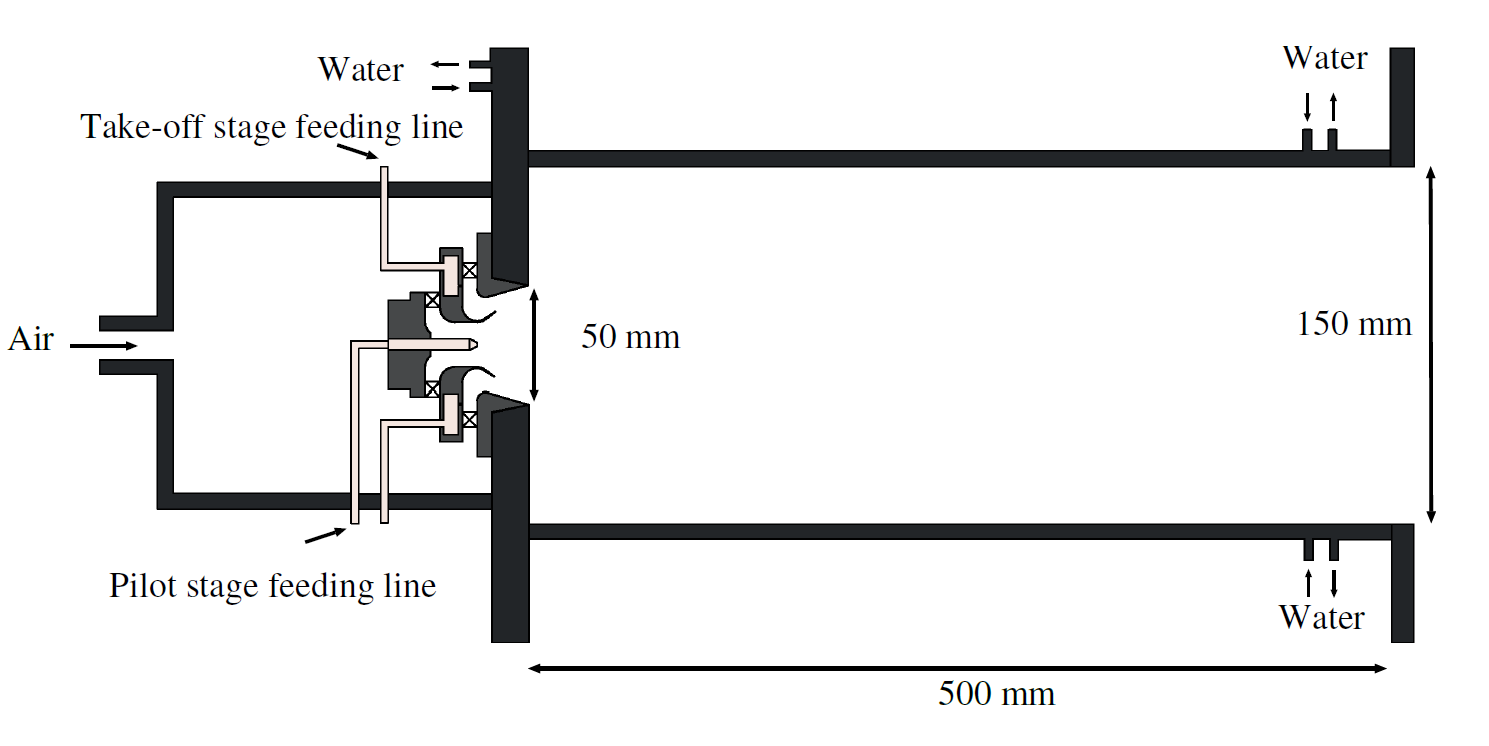
\includegraphics[scale=0.5]{./part3_applications/figures_ch7_aero/BIMER_test_bench_expe_maquette}
	\caption[BIMER experimental test bench]{BIMER experimental test bench. Source: \citeColor[cheneau_etude_2019].}
	\label{fig:BIMER_test_bench_expe_maquette}
\end{figure}

A detailed view of the burner is shown in Figure \ref{fig:BIMER_swirler}. Each stage has a swirler and a liquid injector. The swirlers will give a rotating motion to the air coming from the plenum. The stages are designed as follows:

\begin{itemize}

	\item The \textbf{pilot stage} consists of a swirler with 18 vanes located in a crown with inner and outer diameters of 30 and 45 mm. These vanes have a width of 6 mm and a 42 $\degree$ inclination angle. Fuel injected through the pilot will form a hollow cone.
	
	\item The \textbf{take-off stage} consists of a swirler with 20 vanes of 35 $\degree$ inclination, 10 mm wide spanning between inner and outer diameters of 55 and 75 mm. The swirl number generated is close to 1. Regarding liquid delivery, 10 injection holes with $0.3$ mm diameter are located equally spaced along the multipoint annulus, and with the same radial distance to the center of the pilot injector. Each hole is aligned with the center of a vane (one hole every two vanes), and the vanes are placed so that the swirls of each stage are co-rotating.

\end{itemize}

\begin{figure}[h!]
	\centering
	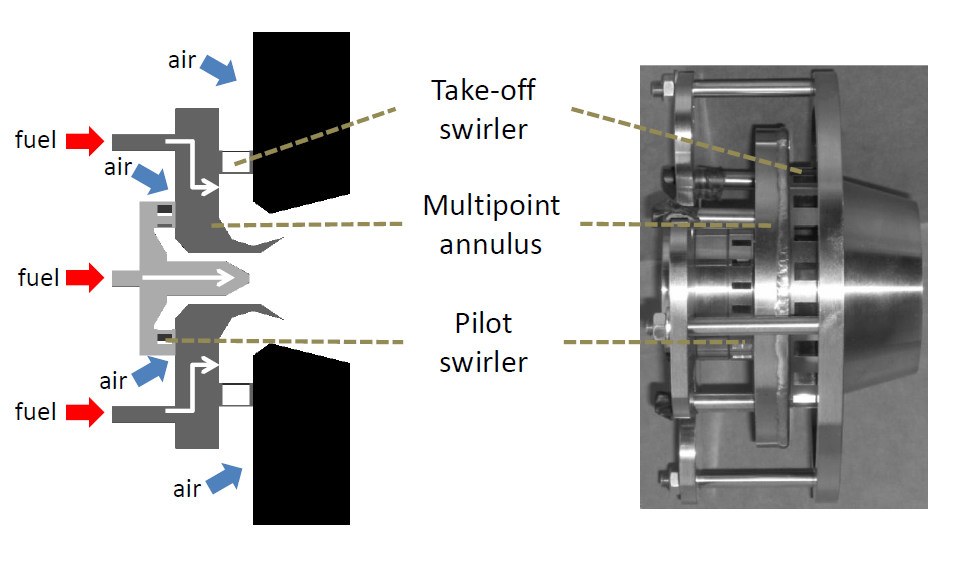
\includegraphics[scale=0.7]{./part3_applications/figures_ch7_aero/BIMER_swirler}
	\caption{Swirled injector of the BIMER test bench. \textsl{Left}: schematic cross-section of the injector, indicating air and liquid inlets. \textsl{Right}: experimental view of the injector. Source: \citeColor[renaud_high-speed_2015].}
	\label{fig:BIMER_swirler}
\end{figure}

The test bench operates at atmospheric pressure. Air can be preheated up to a temperature of $600 K$. The injected fuel through each stage is dodecane. Kerosene was not used since at a laboraty scale it can present risk of coking and its complex chemistry hinders the analysis of the flames \citepColor[providakis_etude_2013]. Hence, dodecane was chosen due to its more simple composition and to its similar properties to kerosene. Dodecane properties of interest for this work are shown in Table \ref{tab:dodecane_properties}.

\begin{table}[!h]
\centering
\caption{Physical properties of dodecane fuel (C$_{12}$H$_26$) at 20 $\degree$C}
\begin{tabular}{|c|c|c|}
\hline
$\rho$ [kg m$^{-3}$]   & $\mu$ [Pa s]   & $\sigma$ [N m$^{-1}$]  \\
\hline
750 & $1.36 \cdot 10^{-3}$ & $22 \cdot 10^{-3}$ \\
\hline
\end{tabular}
\label{tab:dodecane_properties}
\end{table}


\section{Choice of operating points}

Gaseous flow simulations of BIMER have been performed for two operating conditions tested experimentally \citemColor[providakis_etude_2013,renaud_high-speed_2015]. One condition is used for validation of the aerodynamic simulations, while the other is used as application to obtain a developed aerodynamic field for initialising two-phase computations in the next chapters:

\begin{itemize}

	\item \textbf{Validation} of the gaseous simulations is performed with the operating point tested experimentally by \citeColor[providakis_etude_2013], since this one presents data on the non-reactive aerodynamic field. The simulations are also compared to numerical results obtained for this same operating condition by \citeColor[cheneau_etude_2019]. 
	
	\item \textbf{Application} to the setup condition tested by \citeColor[renaud_high-speed_2015]. This study shows data on non-reactive spray characteristics, and hence it will be used as the application case to run the full flowchart formerly introduced in Chapter \ref{ch4:sli_development}. %It is, however, not used for validating the gaseous simulations since it does not present pertinent data.

\end{itemize}

The parameters corresponding to both operating points are listed in Table \ref{tab:gaseous_operating_points_BIMER}. 

\begin{table}[!h]
\centering
\caption{Operating points for performing non-reactive gaseous simulations}
\begin{tabular}{|c|c|c|c|c|c|c|}
\hline
Operating condition    & $\dot{m}_g$ [g s$^{-1}$] & $T_g$ [K] & $\rho_g$ [kg m$^{-3}]$  & $\mu_g$ [Pa s] & $p$ [atm]  & Reference\\
\hline
\hline
Validation &   53 & 473 & 0.746089 & $2.571 \cdot 10^{-5}$ & 1 & \citeColor[providakis_etude_2013]\\
\hline
Application  & 43.1 & 433 & 0.816382 & $2.391 \cdot 10^{-5}$ & 1 & \citeColor[renaud_high-speed_2015] \\
\hline
\end{tabular}
\label{tab:gaseous_operating_points_BIMER}
\end{table}



\section{Numerical setup}


\subsection{Computational geometry}

The computational configuration of the BIMER test bench is shown in Figure \ref{fig:BIMER_geometry_full_domain}. Air is introduced into the plenum through a cylindrical nozzle. The MSFI burner is located at the end of the plenum. A divergent nozzle connected the burner with the combustion chamber. At the end of the chamber, a region representing the atmosphere is located with a coflow of air at low speed ($5$ m/s) and the outlet of the domain.  

\begin{figure}[h!]
	\centering
	\includeinkscape[inkscapelatex=false,scale=0.25]{./part3_applications/figures_ch7_aero/BIMER_geometry_full_domain}
	\caption{Numerical configuration of BIMER test bench}
	\label{fig:BIMER_geometry_full_domain}
\end{figure}

Figure \ref{fig:BIMER_geometry_flower_details} gives a detailed view of the MSFI burner. Both the take-off and pilot stages are represented as in the experimental geometry, with the fuel injectors and the gaseous swirlers. Fuel feeding lines and other represented have not been modeled due to their geometrical complexity \citepColor[cheneau_etude_2019]. The flower, whose main function is to fix the burner to the test rig, has been included in the computational domain since it may affect the incoming gaseous field.

\begin{figure}[h!]
	\centering
	\includeinkscape[inkscapelatex=false,scale=0.25]{./part3_applications/figures_ch7_aero/BIMER_geometry_flower_details}
	\caption[Details of multipoint injector from BIMER test bench.]{Details of multipoint injector from BIMER test bench. \textsl{Left}: side view indicating same features of Figure \ref{fig:BIMER_swirler}. \textsl{Right}: isometric view of the injector, with a zoom-in region showing the multipoint injector.}
	\label{fig:BIMER_geometry_flower_details}
\end{figure}

\subsection{Meshes}

About the meshes, the two used are (see .tex file): %\textbf{mesh_31e6_face_sizing.msh} (bad) and \textbf{mesh_37e6.msh} (good, last mesh)

Steps to follow (for this section):

\begin{enumerate}
	
	\item \textbf{DONE} Show numerical domain with dimensions (as done in JICF, with a similar geometry to the one by Cheneau 2019).
	
	\item Recover meshes (all, including Vie). Give details on the two (or three) meshes I've used. Mention that we are gonna compare with the meshes by Aymeric (i.e. Cheneau).
	
	\item Maybe give details on the parameters/boundary conditions ?

\end{enumerate}



\section{Validation of gaseous field}

Steps to follow (for this section):

\begin{enumerate}
	
	\item Recover both simulations for Providakis with all meshes used.
	
	\item Show mean field (velocities, indicate, IRZ, ORZ, vortical structures ...) for finest simulation
	
	\item \textbf{Qualitative results}: show validation with finest simulation.
	
	\item \textbf{Quantitative results}: show validation with all simulations (two meshes used Y2, results by Cheneau, and results obtained with the meshes of Aymeric).
	

\end{enumerate}

Results are contained here: $Ongoing - BIMER - postprocessing - aero$. They were discussed in the pilotage of 16 March 2021.

%Show nice streamlines (Fig. 6.4 Esclapez-1) and PVC. It would be nice to compare them for both operating conditions

\begin{figure}[h!]
	\centering
	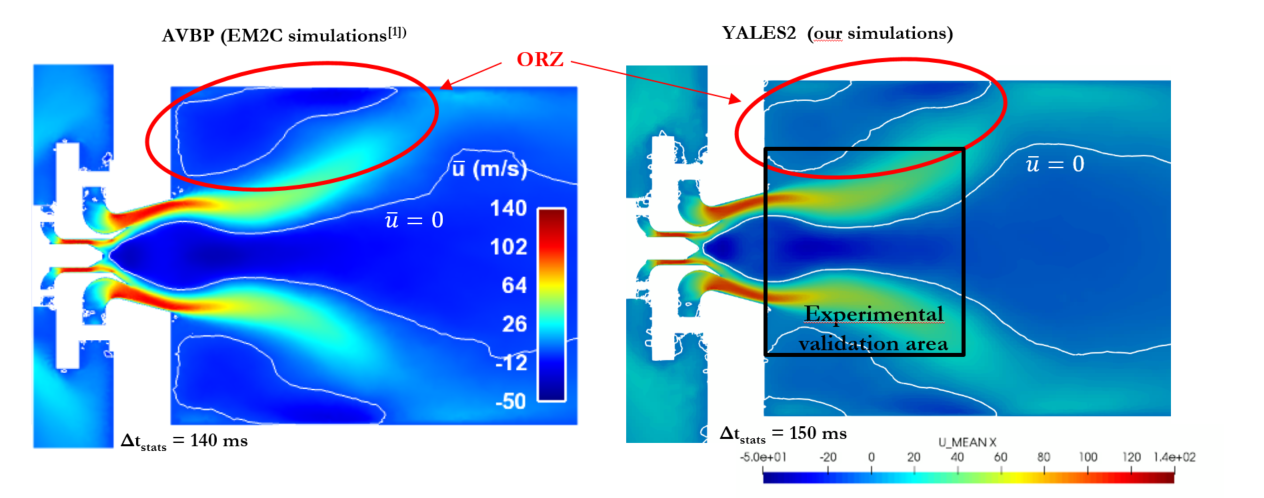
\includegraphics[scale=0.7]{./part3_applications/figures_ch7_aero/quantitative_view_mean_velocity_field}
	\caption{Mean velocity field .}
	\label{fig:quantitative_view_mean_velocity_field}
\end{figure}

\subsection{Mesh independence study}


\subsection{Qualitative validation}


See Figure \ref{fig:validation_qualitative_u}: \ref{fig:validation_qualitative_u_mean} and \ref{fig:validation_qualitative_u_rms}.


\begin{figure}
\centering
\begin{subfigure}[b]{1.0\textwidth}
	\centering
   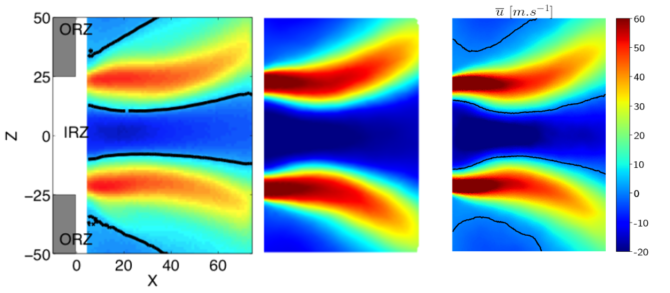
\includegraphics[scale=1.0]{./part3_applications/figures_ch7_aero/validation_qualitative_u_mean}
   \caption{Mean axial velocity}
   \label{fig:validation_qualitative_u_mean} 
\end{subfigure}
\begin{subfigure}[b]{1.0\textwidth}
	\centering
   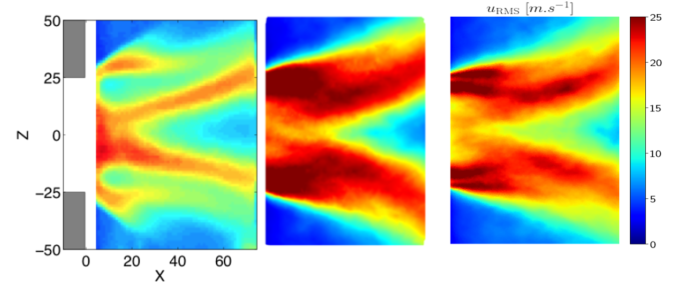
\includegraphics[scale=1.0]{./part3_applications/figures_ch7_aero/validation_qualitative_u_rms}
   \caption{RMS axial velocity}
   \label{fig:validation_qualitative_u_rms}
\end{subfigure}
\caption{Fields of axial velocity in enclosed region from Figure \ref{fig:quantitative_view_mean_velocity_field}. \textsl{Left}: experimental results. \textsl{Center}: numerical results obtained by \citeColor[cheneau_etude_2019]. \textsl{Right}: results from present work.}
\label{fig:validation_qualitative_u}
\end{figure}

\begin{figure}
\centering
\begin{subfigure}[b]{1.0\textwidth}
	\centering
   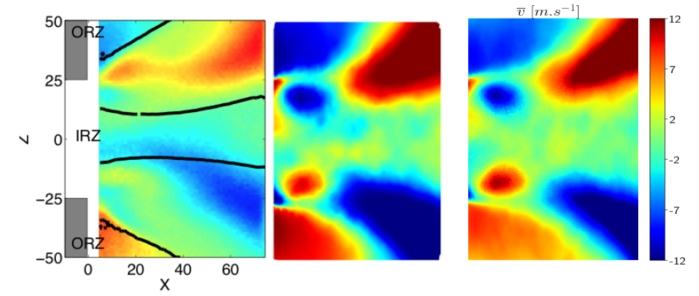
\includegraphics[scale=1.0]{./part3_applications/figures_ch7_aero/validation_qualitative_v_mean}
   \caption{Mean vertical velocity}
   \label{fig:validation_qualitative_v_mean} 
\end{subfigure}
\begin{subfigure}[b]{1.0\textwidth}
	\centering
   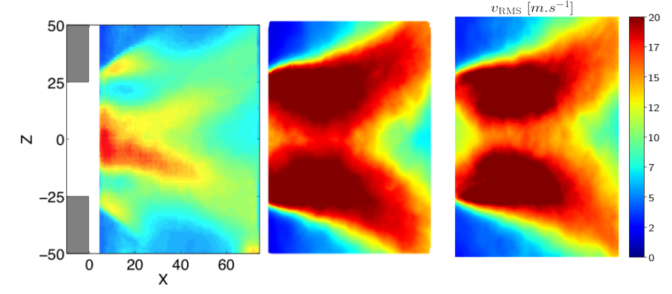
\includegraphics[scale=1.0]{./part3_applications/figures_ch7_aero/validation_qualitative_v_rms}
   \caption{RMS vertical velocity}
   \label{fig:validation_qualitative_v_rms}
\end{subfigure}
\caption{Fields of vertical velocity in enclosed region from Figure \ref{fig:quantitative_view_mean_velocity_field}. \textsl{Left}: experimental results. \textsl{Center}: numerical results obtained by \citeColor[cheneau_etude_2019]. \textsl{Right}: results from present work.}
\label{fig:validation_qualitative_v}
\end{figure}





\subsection{Quantitative validation}

\section{Application point}
	\label{ch7:BIMER_application_point}

Steps to follow (for this section):

\begin{enumerate}
	
	\item Take the only simulation performed (with finest mesh).
	
	\item Show mean field, velocity field.
	
	\item Show PVC, vortical structures, try to get some interesting results (get inspired by Esclapez, for example).
	

\end{enumerate}


\section{Conclusion}

%\section{Validation (Providakis 2013)}
%
%
%\subsection{Quantitative data}
%
%\subsection{Qualitative data}
%
%\section{Application (Renaud 2015)}
%
